\chapter{涨落、相变与集体现象}

\begin{prereqbox}
熟悉热力学基本关系、正则分布和 Bose/Fermi 分布。本章把“会写分布函数”推进到“会从配分函数求响应、会判断相变、会连接电子和声子实验”。
\end{prereqbox}
\begin{mapbox}
\[
\ln Z\to\text{热力学势}\to\text{平均值与涨落}\to\text{响应函数},
\]
\[
\text{对称性}+\text{序参量}\to\text{Landau 理论}\to
\text{临界现象与量子相变}.
\]
\end{mapbox}

\section{熵最大原理与系综}
在给定归一化和平均能量约束时最大化
\[
S=-\kb\sum_i p_i\ln p_i
\]
的 Lagrange 泛函：
\[
\mathcal L=-\kb\sum_i p_i\ln p_i
-\alpha\left(\sum_i p_i-1\right)
-\tilde\beta\left(\sum_i p_iE_i-U\right).
\]
令 $\partial\mathcal L/\partial p_i=0$ 得
$p_i\propto e^{-\beta E_i}$。热库推导说明 $\beta=1/\kb T$，最大熵推导说明正则分布是在已知平均能量时最少偏置的分布。两种论证互补。

巨正则配分函数
\[
\Xi=\mathrm{Tr}\,\ee^{-\beta(H-\mu N)},\qquad
\Omega=-\kb T\ln\Xi.
\]
由微分
$\dd\Omega=-S\dd T-P\dd V-N\dd\mu$ 得
\[
N=-\left(\pdv{\Omega}{\mu}\right)_{T,V},\qquad
P=-\left(\pdv{\Omega}{V}\right)_{T,\mu}.
\]
开放粒子数问题、量子气体和二次量子化 Hamiltonian 最适合使用巨正则系综。

\section{涨落与响应}
正则系综中
\[
\langle E\rangle=-\pdv{\ln Z}{\beta},\qquad
\frac{\partial^2\ln Z}{\partial\beta^2}
=\langle E^2\rangle-\langle E\rangle^2.
\]
因此
\[
\boxed{\langle(\Delta E)^2\rangle=\kb T^2C_V}.
\]
宏观系统中 $E\sim N$、涨落标准差 $\sim\sqrt N$，相对涨落 $\sim N^{-1/2}$，这解释了热力学量为何看起来确定。

若 Hamiltonian 含外场 $H=H_0-hA$，则
\[
\langle A\rangle=\frac1\beta\pdv{\ln Z}{h},
\qquad
\pdv{\langle A\rangle}{h}
=\beta\left(\langle A^2\rangle-\langle A\rangle^2\right).
\]
响应等于平衡涨落，是涨落-耗散思想的静态版本。磁化率对应磁矩涨落，压缩率对应粒子数或体积涨落。

\begin{examplebox}
\textbf{二能级 Schottky 热容。}能级为 $0,\Delta$，配分函数
$Z=1+e^{-\beta\Delta}$。平均能量
\[
U=\frac{\Delta}{e^{\beta\Delta}+1},
\]
于是
\[
C=\kb(\beta\Delta)^2\frac{e^{\beta\Delta}}
{(1+e^{\beta\Delta})^2}.
\]
$T\to0$ 时激发冻结，$T\to\infty$ 时两能级等占据且能量趋于常数，所以两端热容都为零，中间出现 Schottky 峰。
\end{examplebox}

\section{理想 Fermi 气与 Sommerfeld 展开}
积分
\[
I=\int_0^\infty\phi(E)f(E)\dd E
\]
在 $\kb T\ll E_F$ 时可展开为
\[
I=\int_0^\mu\phi(E)\dd E
+\frac{\pi^2}{6}(\kb T)^2\phi'(\mu)+O(T^4).
\]
证明的核心是把 $f(E)-\Theta(\mu-E)$ 局域在 $\mu$ 附近，并利用其奇偶矩。固定粒子数后
\[
\mu(T)=E_F\left[1-\frac{\pi^2}{12}
\left(\frac{\kb T}{E_F}\right)^2+\cdots\right],
\]
\[
U(T)=U(0)+\frac{\pi^2}{6}g(E_F)(\kb T)^2,
\qquad C_V=\frac{\pi^2}{3}\kb^2g(E_F)T.
\]
金属低温比热常写
\[
\frac CT=\gamma+\beta T^2,
\]
截距 $\gamma$ 来自电子，斜率 $\beta$ 来自 Debye 声子。实验上由此可估算态密度和 Debye 温度。

\section{理想 Bose 气与凝聚}
固定粒子数时
\[
N=\sum_{\vb k}\frac1{e^{\beta(\epsilon_k-\mu)}-1},
\qquad \mu\le\epsilon_0.
\]
三维自由粒子激发态能容纳的最大粒子数为
\[
N_{\rm ex}^{\max}
=\frac{V}{\lambda_T^3}\zeta(3/2).
\]
当总粒子数超过它，多余粒子宏观占据基态，临界温度
\[
T_c=\frac{2\pi\hbar^2}{m\kb}
\left[\frac{n}{\zeta(3/2)}\right]^{2/3}.
\]
声子虽然服从 Bose 统计，却因数目不守恒而通常取 $\mu=0$；它们的低温性质来自线性色散，不等同于有质量玻色气体凝聚。

\section{Landau 理论、关联长度与临界指数}
对满足 $m\to-m$ 对称性的序参量，
\[
F[m]=F_0+\int\dd^dr\left[
\frac\kappa2(\nabla m)^2+\frac a2(T-T_c)m^2+\frac b4m^4-hm
\right].
\]
均匀、零场时极值满足
\[
a(T-T_c)m+bm^3=0.
\]
$T<T_c$ 有
$m_0=\pm\sqrt{a(T_c-T)/b}$，故平均场指数 $\beta_{\rm MF}=1/2$。
在 $T>T_c$ 的小外场线性响应
\[
\chi=\pdv mh=\frac1{a(T-T_c)},
\]
给 $\gamma_{\rm MF}=1$。考虑空间起伏并线性化，
\[
[-\kappa\nabla^2+a(T-T_c)]m=h,
\]
Fourier 空间
$\chi(q)=1/[\kappa q^2+a(T-T_c)]$，定义
\[
\xi=\sqrt{\frac{\kappa}{a|T-T_c|}},
\]
故 $\nu_{\rm MF}=1/2$。临界点附近 $\xi$ 发散，涨落跨越许多尺度，正是简单平均场失效的原因。

\begin{figure}[htbp]
\centering
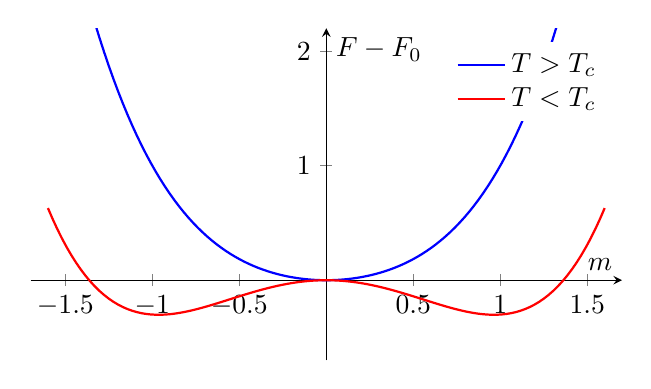
\begin{tikzpicture}
\begin{axis}[width=0.75\textwidth,height=5.8cm,
xlabel={$m$},ylabel={$F-F_0$},axis lines=middle,
xmin=-1.7,xmax=1.7,ymin=-0.7,ymax=2.2,samples=120,
legend style={draw=none,at={(0.98,0.96)},anchor=north east}]
\addplot[blue,thick,domain=-1.6:1.6] {0.65*x^2+0.35*x^4};
\addlegendentry{$T>T_c$}
\addplot[red,thick,domain=-1.6:1.6] {-0.65*x^2+0.35*x^4};
\addlegendentry{$T<T_c$}
\end{axis}
\end{tikzpicture}
\caption{Landau 自由能从单阱变为双阱，展示序参量的自发选择。}
\end{figure}

\begin{whybox}
为什么必须先确定序参量和对称性？Landau 展开允许的项由对称性决定。铁磁体零场下有 $m\to-m$，不能出现奇次项；若外场非零，$-hm$ 显式破坏该对称性。密度波序参量通常是复数，其相位对应平移；超导序参量也是复数，但还与电磁规范耦合。
\end{whybox}

\section{经典相变与量子相变}
经典连续相变由温度驱动，临界涨落主要是热涨落。量子相变发生在 $T=0$，由压力、磁场、掺杂或相互作用强度等非热参数调控，涨落来自不确定性。虚时间路径积分把 $d$ 维量子系统映射到额外含时间维的经典问题，动态临界指数 $z$ 描述
\[
\xi_\tau\sim\xi^z.
\]
有限温度会截断虚时间长度 $\hbar/\kb T$，在量子临界扇区产生非费米液体或非常规标度。面试中不必背所有指数，但要区分“零温基态重排”和普通热相变。

\section{线性响应与 Kubo 公式的物理结构}
若外扰
$H'(t)=-f(t)B$，一阶响应
\[
\delta\langle A(t)\rangle
=\int_{-\infty}^{t}\chi_{AB}(t-t')f(t')\dd t',
\]
\[
\boxed{\chi_{AB}(t)=\frac{i}{\hbar}\theta(t)
\langle[B(0),A(t)]\rangle_0}.
\]
$\theta(t)$ 保证因果性；对易子反映量子涨落。频域中响应的实部常描述色散，虚部描述吸收。电导率、磁化率、介电函数和散射谱都可以放入这一框架。静态涨落-响应关系是它在低频平衡极限的影子。

\section{三个完整例题}
\begin{examplebox}
\textbf{例 1：顺磁自旋的涨落。}对 $N$ 个独立 Ising 磁矩
$m_i=\pm\mu$，零场 $\langle M\rangle=0$，
$\langle M^2\rangle=N\mu^2$。涨落-响应给
\[
\chi=\beta\langle M^2\rangle/V
=\frac{n\mu^2}{\kb T},
\]
即 Curie 定律。平均场加入有效场反馈后变为 Curie-Weiss 形式。
\end{examplebox}

\begin{examplebox}
\textbf{例 2：一维经典 Ising 为何无有限温铁磁序？}产生一个畴壁代价有限能量
$\Delta E=2J$，但畴壁可放在约 $N$ 个位置，熵增
$\Delta S\simeq\kb\ln N$。任意 $T>0$ 下大系统的
$\Delta F=2J-\kb T\ln N$ 最终为负，畴壁增殖破坏长程有序。
\end{examplebox}

\begin{examplebox}
\textbf{例 3：由低温比热分离电子和声子。}若实验拟合
$C/T=\gamma+\beta T^2$，作 $C/T$ 对 $T^2$ 图，截距为 $\gamma$；由
\[
\beta=\frac{12\pi^4}{5}\frac{N\kb}{\Theta_D^3}
\]
可估算 $\Theta_D$。若低温出现指数衰减或跳变，则可能提示超导能隙或相变。
\end{examplebox}

\section{面试总结与自测}
\begin{interviewbox}
\textbf{配分函数为什么重要？}它是带权微观态计数，也是热力学量的生成函数；一阶导数给平均值，二阶导数给涨落和响应。回答时应给
$F=-\kb T\ln Z$、$U=-\partial_\beta\ln Z$ 与
$\langle(\Delta E)^2\rangle=\kb T^2C_V$ 三层关系。

\textbf{量子相变与经典相变有何不同？}先说驱动参数和涨落来源，再说有限温交叉和动态指数，不要把“发生在低温”当定义。
\end{interviewbox}
\begin{selftestbox}
\begin{enumerate}
\item 用最大熵法推导巨正则分布。
\item 推导能量涨落与热容关系，并估算相对涨落尺度。
\item 化学势在 Bose 与 Fermi 系统中的约束有何不同？
\item Sommerfeld 展开的适用条件是什么？
\item 为什么金属低温常画 $C/T$ 对 $T^2$？
\item 从 Landau 自由能求 $\beta_{\rm MF},\gamma_{\rm MF}$。
\item 梯度项如何定义关联长度？
\item 为什么一维短程 Ising 模型没有有限温相变？
\item Kubo 响应函数中的阶跃函数有何意义？
\item 声子、磁振子、电子分别服从什么统计，化学势如何处理？
\end{enumerate}
\end{selftestbox}
